\subsection{Opgave 50}

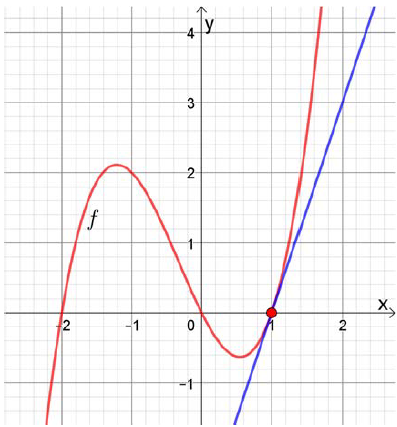
\includegraphics[width=8cm]{Opgave_41-50/Opgave_50/50.png}

Figuren viser grafen for en funktion f og dens tagnet i $x = 1$.

Benyt figuren til at bestemme $f'(1)$.

\ans

For at bestemme $f'(1)$ skal vi altså bestemme hældningen for $f(x)$ i det punkt hvor $x = 1$. Da vi også er givet tangenten til 
$f(x)$ i $x = 1$ og da hældningen på tangenten i $x = 1$ og $f'(1)$ er det samme kan vi altså aflæse tangentens hældning.

Da tangenten er en ret linje, kan vi aflæse den hældning ved at gå 1 hen ad x aksen, og så op af y aksen indtil vi rammer tangenten igen.
Det stykke vi bevæger os op vil så svare til tangentens hældning og dermed $f'(1)$. Går vi en hen ad x aksen skal vi bevægge os 3 op ad y aksen
før vi rammer tangenten igen. Hældningen på tangenten er dermed 3 og derfor er $f'(1) = 3$. Figuren nedenfor viser aflæsningen af tangentens hældning.

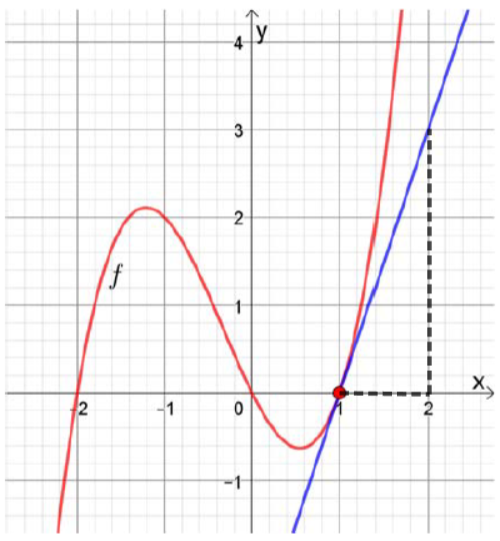
\includegraphics[width=8cm]{Opgave_41-50/Opgave_50/50.1.png}